\chapter{Google V8 Javascriptengine}
\label{cha:v8engine}

Während im letzten Kapitel auf die Konzepte und Funktionsweise von SCADA-Systemen eingegangen wurde, widmet sich dieses nun der Skriptsprache Javascript. 
Es wird gezeigt, wie diese Sprache technisch funktioniert. Als Javascriptengine bezeichnet man Programmkomponenten, die ECMA standardkonformen Quellcode ausführen können \cite{ecma}. 
Danach werden die drei bekanntesten Engines verglichen, um zu erläutern, warum die Google-V8-Engine für die Umsetzung gewählt wurde. 
Im letzten Abschnitt wird die Programmierschnittstelle dieser beschrieben. 

\section{Grundlagen}

Um zu verstehen, wie Javascript-Engines funktionieren, müssen die Grundlagen der Compilertheorie umrissen werden. Dazu wird
hier nun Bezug auf \cite{dragonBook} genommen. Als Compiler bezeichnet man ein Programm, das von Menschen lesbaren Quellcode
in binären Programmcode umwandelt, der von einem Computer ausgeführt werden kann. Im Folgenden wird die Theoretische
Funktionsweise eines solchen Programms beschrieben. 

, \cite{jsCore}, \cite{v8ByteCode}, \cite{jsSpiderMonkey}
Bevor das Umsetzungskonzept erläutert werden kann, muss die generelle Funktionsweise der Google V8 Javascriptengine
erörtert werden. Dazu wird in diesem Abschnitt Bezug auf \cite{v8embed} und \cite{v8mem} genommen.

\subsection{Contexts}

Ein Context ist eine Ausfuhrungsumgebung, die es ermöglicht, separaten, unabhängigen Javascript-Code in einer einzigen 
V8-Instanz (Isolate) auszufuhren. Da eine Isolate mehrere Context-Ausführungsumgebungen besitzen kann, muss jene, die zur 
Ausführung verwendet werden soll explizit angegeben werden. In dem Webbrowser \textit{Chromium} wird das Konzept der 
Contexts für je ein HTML Fenster oder \textit{iframe} verwendet.

\begin{figure}[h]
	\centering 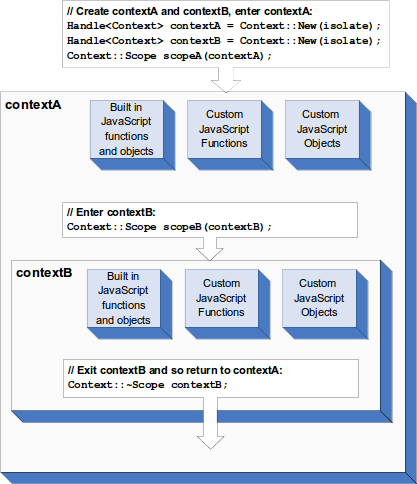
\includegraphics[width=0.7\textwidth]{contexts}
	\caption{In dieser Illustration wird die Unabhängigkeit der verschiedenen Contexts zueinander veranschaulicht.}
	\label{fig:contexts}
\end{figure}

In Abbildung \ref{fig:contexts} ist außerdem ersichtlich, dass mehrere Contexts auch verschachtelt aufgerufen 
werden können ohne sich gegenseitig zu beeinflussen.

\begin{figure}[h]
	\centering 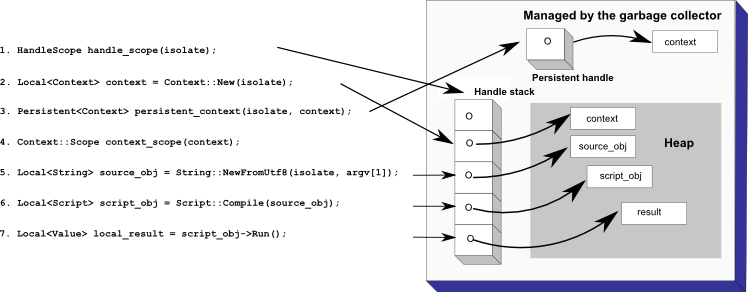
\includegraphics[width=1\textwidth]{handles}
	\caption{}
	\label{fig:handles}
\end{figure}

Jens

\section{Funktionsweise und Aufbau}

\subsection{Just-In-Time Compiler und Caches}

\subsection{Threadsicherheit mithilfe von Isolates}

1 Thread per Isolate, Locker Objekte

\subsection{Abgrenzen der Javascript-Ausführungsumgebungen mithilfe von Contexts}

Unabhängige ausführungsumgebung

\subsection{Speicherverwaltung}

Handles verwaltet über RAII geben Garbage collector auskunft über die validität von speicherzellen.

\subsection{Anpassen von Javascript-Ausführungsumgebungen über das Global Objekt}

\subsection{Das DebugInspector Protokoll}

\section{Vergleich mit anderen Javascript-Engines}
Vergleich vorallem mid Mozilla spidermonkey. Ev. auch performancetests.
\subsection{Mozilla SpiderMonkey}


\subsection{Apple JavaScriptCore}

